% move all configuration stuff into includes file so we can focus on the content
\documentclass[aspectratio=169,hyperref={pdfpagelabels=false,colorlinks=true,linkcolor=white,urlcolor=gtgold},t]{beamer}

%%%%%%%%%%%%%%%%%%%%%%%%%%%%%%%%%%%%%%%%%%%%%%%%%%%%%%%%%%%%%%%%%%%%%%%%%%%%%%%%%%
%%%%%%%%%%%%%%%%%%%%%%%%%%%%%%%%%%%%%%%%%%%%%%%%%%%%%%%%%%%%%%%%%%%%%%%%%%%%%%%%%%
% packages
\usepackage{pict2e}
\usepackage{epic}
\usepackage{amsmath,amsfonts,amssymb}
\usepackage{units}
\usepackage{fancybox}
\usepackage[absolute,overlay]{textpos} 
%\usepackage{media9} % avi2flv: "C:\Program Files\ffmpeg\bin\ffmpeg.exe" -i TuneFreqFilterbank.avi -b 600k -s 441x324 -r 15 -acodec copy TuneFreqFilterbank.flv
\usepackage{animate}
\usepackage{gensymb}
\usepackage{multirow}
\usepackage{silence}
%\usepackage{tikz}
\usepackage[backend=bibtex,style=ieee]{biblatex}
\AtEveryCitekey{\iffootnote{\tiny}{}}
\addbibresource{include/references}
\addbibresource{include/lerch}
\renewcommand*{\bibfont}{\tiny}



% fontsize
\let\Tiny=\tiny

%%%%%%%%%%%%%%%%%%%%%%%%%%%%%%%%%%%%%%%%%%%%%%%%%%%%%%%%%%%%%%%%%%%%%%%%%%%%%%%%%%
%%%%%%%%%%%%%%%%%%%%%%%%%%%%%%%%%%%%%%%%%%%%%%%%%%%%%%%%%%%%%%%%%%%%%%%%%%%%%%%%%%
% warnings
\pdfsuppresswarningpagegroup=1
\WarningFilter{biblatex}{Patching footnotes failed}
\WarningFilter{latexfont}{Font shape}
\WarningFilter{latexfont}{Some font shapes}
\WarningFilter{gensymb}{Not defining}


%%%%%%%%%%%%%%%%%%%%%%%%%%%%%%%%%%%%%%%%%%%%%%%%%%%%%%%%%%%%%%%%%%%%%%%%%%%%%%%%%%
%%%%%%%%%%%%%%%%%%%%%%%%%%%%%%%%%%%%%%%%%%%%%%%%%%%%%%%%%%%%%%%%%%%%%%%%%%%%%%%%%%
% theme & layout
\usetheme{Frankfurt}
\useinnertheme{rectangles}


%%%%%%%%%%%%%%%%%%%%%%%%%%%%%%%%%%%%%%%%%%%%%%%%%%%%%%%%%%%%%%%%%%%%%%%%%%%%%%%%%%
\setbeamertemplate{frametitle}[default][colsep=-4bp,rounded=false,shadow=false]
\setbeamertemplate{frametitle}
{%
    \nointerlineskip%
    \begin{beamercolorbox}[wd=\paperwidth,ht=3.5ex,dp=0.6ex]{frametitle}
        \hspace*{1.3ex}\insertframetitle%
        
        \hspace*{1.3ex}\small\insertframesubtitle%
    \end{beamercolorbox}%
    %\begin{textblock*}{100mm}(11.6cm,.57cm)
        %\includegraphics[height=.8cm,keepaspectratio]{graph/Logo_GTCMT_white}
    %\end{textblock*}
}


%%%%%%%%%%%%%%%%%%%%%%%%%%%%%%%%%%%%%%%%%%%%%%%%%%%%%%%%%%%%%%%%%%%%%%%%%%%%%%%%%%
\setbeamertemplate{title page}[default][colsep=-4bp,rounded=false,shadow=false]
\setbeamertemplate{title page}
{
    \begin{textblock*}{200mm}(13.5cm,.5cm)
            \href{https://www.\repolink}{
\includegraphics[height=2cm,keepaspectratio]{graph/qr}}\hspace*{2ex}
    \end{textblock*}
    \vskip-10ex
    \begin{beamercolorbox}[wd=\paperwidth,ht=.7\paperheight,dp=0.6ex]{frametitle} %35ex
        \hspace*{1.8ex}\LARGE\inserttitle%
        
        \vspace*{.5ex}
        
        \hspace*{1.3ex}\small\insertsubtitle%
        
        \vspace*{.5ex}
    \end{beamercolorbox}%
    \nointerlineskip%
    \begin{beamercolorbox}[wd=\paperwidth,ht=.4\paperheight,dp=0.6ex]{page number in head/foot}
        %\vspace*{-.5ex}
        \hspace*{1.7ex}\small\insertauthor%
        
        %\hspace*{1.7ex}\small }%
        
        \vspace*{10ex}
        
        %\begin{flushright}
            %\href{http://www.gtcmt.gatech.edu}{\includegraphics[height=.8cm,keepaspectratio]{graph/Logo_GTCMT_black}}\hspace*{2ex}
        %\end{flushright}
    \end{beamercolorbox}%
    \nointerlineskip%
    \begin{beamercolorbox}[wd=\paperwidth,ht=.2\paperheight,dp=0.6ex]{page number in head/foot}
    \end{beamercolorbox}%
	\addreference{\hspace{48mm}\href{https://\repolink}{\repolink}}
}


%%%%%%%%%%%%%%%%%%%%%%%%%%%%%%%%%%%%%%%%%%%%%%%%%%%%%%%%%%%%%%%%%%%%%%%%%%%%%%%%%%
%\makeatother
\setbeamertemplate{footline}
{
  \leavevmode%
  \hbox{%
  \begin{beamercolorbox}[wd=.5\paperwidth,ht=2.25ex,dp=1ex,left,leftskip=1ex]{page number in head/foot}%
    \MakeLowercase\inserttitle
  \end{beamercolorbox}%
  \begin{beamercolorbox}[wd=.5\paperwidth,ht=2.25ex,dp=1ex,right,rightskip=1ex]{page number in head/foot}%
    \hfill
    \insertframenumber{} / \inserttotalframenumber
  \end{beamercolorbox}}%
  \vskip0pt%
}
%\makeatletter


%%%%%%%%%%%%%%%%%%%%%%%%%%%%%%%%%%%%%%%%%%%%%%%%%%%%%%%%%%%%%%%%%%%%%%%%%%%%%%%%%%
\beamertemplatenavigationsymbolsempty
\setbeamertemplate{navigation symbols}{}
\setbeamertemplate{blocks}[default]%[rounded=false,shadow=false]
\setbeamertemplate{itemize item}[square]
\setbeamertemplate{itemize subitem}[circle]
\setbeamertemplate{itemize subsubitem}[triangle]
\setbeamertemplate{enumerate item}[square]
\setbeamertemplate{enumerate subitem}[circle]
\setbeamertemplate{enumerate subsubitem}[circle]


%%%%%%%%%%%%%%%%%%%%%%%%%%%%%%%%%%%%%%%%%%%%%%%%%%%%%%%%%%%%%%%%%%%%%%%%%%%%%%%%%%
% colors
\setbeamercolor{structure}{fg=darkgray}
\setbeamercovered{transparent} %invisible
\setbeamercolor{bibliography entry author}{fg=black}
\setbeamercolor*{bibliography entry title}{fg=black}
\setbeamercolor*{bibliography entry note}{fg=black}
\setbeamercolor{frametitle}{fg=black}
\setbeamercolor{title}{fg=white}
\setbeamercolor{subtitle}{fg=white}
\setbeamercolor{frametitle}{fg=white}
\setbeamercolor{framesubtitle}{fg=white}
\setbeamercolor{mini frame}{fg=white, bg=black}
\setbeamercolor{section in head/foot}{fg=white, bg=darkgray}
\setbeamercolor{page number in head/foot}{fg=black, bg=gtgold}
\setbeamercolor{item projected}{fg=white, bg=black}
\setbeamercolor{section in toc}{fg=black, bg=gtgold}
\setbeamercolor{subsection in toc}{fg=darkgray, bg=gtgold}
%---------------------------------------------------------------------------------
%%%%%%%%%%%%%%%%%%%%%%%%%%%%%%%%%%%%%%%%%%%%%%%%%%%%%%%%%%%%%%%%%%%%%%%%%%%%%%%%%%
%%%%%%%%%%%%%%%%%%%%%%%%%%%%%%%%%%%%%%%%%%%%%%%%%%%%%%%%%%%%%%%%%%%%%%%%%%%%%%%%%%
% title information
%\title[]{Introduction to Audio Content Analysis}   
\author[alexander lerch]{alexander lerch} 
%\institute{~}
%\date[Alexander Lerch]{}
%\titlegraphic{\vspace{-16mm}\includegraphics[width=\textwidth,height=3cm]{title}}

%%%%%%%%%%%%%%%%%%%%%%%%%%%%%%%%%%%%%%%%%%%%%%%%%%%%%%%%%%%%%%%%%%%%%%%%%%%%%%%%%%
%%%%%%%%%%%%%%%%%%%%%%%%%%%%%%%%%%%%%%%%%%%%%%%%%%%%%%%%%%%%%%%%%%%%%%%%%%%%%%%%%%
% colors
\definecolor{gtgold}{HTML}{E0AA0F} %{rgb}{0.88,0.66,1,0.06} [234, 170, 0]/256
\definecolor{darkgray}{rgb}{.2,.2,.2}
%\definecolor{gtgold_less}{rgb}{.88,0.66,0} %_less!40
\definecolor{highlight}{HTML}{E0AA0F}

%%%%%%%%%%%%%%%%%%%%%%%%%%%%%%%%%%%%%%%%%%%%%%%%%%%%%%%%%%%%%%%%%%%%%%%%%%%%%%%%%%
%%%%%%%%%%%%%%%%%%%%%%%%%%%%%%%%%%%%%%%%%%%%%%%%%%%%%%%%%%%%%%%%%%%%%%%%%%%%%%%%%%
% relative paths (change 2nd path to pull dir of https://github.com/alexanderlerch/ACA-Plots)
\graphicspath{{./graph/}{../../ACA/ACA-Plots/graph/}}

%%%%%%%%%%%%%%%%%%%%%%%%%%%%%%%%%%%%%%%%%%%%%%%%%%%%%%%%%%%%%%%%%%%%%%%%%%%%%%%%%%
%%%%%%%%%%%%%%%%%%%%%%%%%%%%%%%%%%%%%%%%%%%%%%%%%%%%%%%%%%%%%%%%%%%%%%%%%%%%%%%%%%
% links
\def\repolink{github.com/alexanderlerch/\jobname}


%%%%%%%%%%%%%%%%%%%%%%%%%%%%%%%%%%%%%%%%%%%%%%%%%%%%%%%%%%%%%%%%%%%%%%%%%%%%%%%%%%
%%%%%%%%%%%%%%%%%%%%%%%%%%%%%%%%%%%%%%%%%%%%%%%%%%%%%%%%%%%%%%%%%%%%%%%%%%%%%%%%%%
% units
\setlength{\unitlength}{1mm}

%%%%%%%%%%%%%%%%%%%%%%%%%%%%%%%%%%%%%%%%%%%%%%%%%%%%%%%%%%%%%%%%%%%%%%%%%%%%%%%%%%
%%%%%%%%%%%%%%%%%%%%%%%%%%%%%%%%%%%%%%%%%%%%%%%%%%%%%%%%%%%%%%%%%%%%%%%%%%%%%%%%%%
% math
\DeclareMathOperator*{\argmax}{argmax}
\DeclareMathOperator*{\argmin}{argmin}
\DeclareMathOperator*{\atan}{atan}
\DeclareMathOperator*{\arcsinh}{arcsinh}
\DeclareMathOperator*{\sign}{sign}
\DeclareMathOperator*{\tcdf}{tcdf}
\DeclareMathOperator*{\si}{sinc}
\DeclareMathOperator*{\princarg}{princarg}
\DeclareMathOperator*{\arccosh}{arccosh}
\DeclareMathOperator*{\hwr}{HWR}
\DeclareMathOperator*{\flip}{flip}
\DeclareMathOperator*{\sinc}{sinc}
\DeclareMathOperator*{\floor}{floor}
\newcommand{\e}{{e}}
\newcommand{\jom}{\mathrm{j}\omega}
\newcommand{\jOm}{\mathrm{j}\Omega}
\newcommand   {\mat}[1]    		{\boldsymbol{\uppercase{#1}}}		%bold
\renewcommand {\vec}[1]    		{\boldsymbol{\lowercase{#1}}}		%bold

%%%%%%%%%%%%%%%%%%%%%%%%%%%%%%%%%%%%%%%%%%%%%%%%%%%%%%%%%%%%%%%%%%%%%%%%%%%%%%%%%%
%%%%%%%%%%%%%%%%%%%%%%%%%%%%%%%%%%%%%%%%%%%%%%%%%%%%%%%%%%%%%%%%%%%%%%%%%%%%%%%%%%
% media9
\newcommand{\includeaudio}[1]{
\href{run:audio/#1.mp3}{
\includegraphics[width=5mm, height=5mm]{graph/icon/SpeakerIcon}}
}
\newcommand{\includevideo}[1]{
\href{run:video/#1}{
\includegraphics[width=20mm, height=20mm]{graph/icon/play_button}}
}

\newcommand{\includeanimation}[4]{{\begin{center}
                        \animategraphics[autoplay,loop,scale=.7]{#4}{animation/#1-}{#2}{#3}        
                        \end{center}
                        \addreference{matlab source: \href{https://github.com/alexanderlerch/ACA-Plots/blob/master/matlab/animate#1.m}{matlab/animate#1.m}}}
                        \inserticon{video}}
                        
%%%%%%%%%%%%%%%%%%%%%%%%%%%%%%%%%%%%%%%%%%%%%%%%%%%%%%%%%%%%%%%%%%%%%%%%%%%%%%%%%%
%%%%%%%%%%%%%%%%%%%%%%%%%%%%%%%%%%%%%%%%%%%%%%%%%%%%%%%%%%%%%%%%%%%%%%%%%%%%%%%%%%
% other commands
\newcommand{\question}[1]{%\vspace{-4mm}
                          \setbeamercovered{invisible}
                          \begin{columns}[T]
                            \column{.9\textwidth}
                                \textbf{#1}
                            \column{.1\textwidth}
                                \vspace{-8mm}
                                \begin{flushright}
                                     \includegraphics[width=\columnwidth]{graph/question_mark}
                                \end{flushright}
                                \vspace{6mm}
                          \end{columns}\pause\vspace{-12mm}}

\newcommand{\toremember}[1]{%\vspace{-4mm}
                          %\begin{columns}[T]
                            %\column{.8\textwidth}
                                %\textbf{#1}
                            %\column{.2\textwidth}
                                %\vspace{-4mm}
                                %\begin{flushright}
                                     %\includegraphics[scale=.5]{exclamation_mark}
                                %\end{flushright}
                                %\vspace{6mm}
                          %\end{columns}\vspace{-6mm}
                        \inserticon{lightbulb}
                        }

\newcommand{\matlabexercise}[1]{%\vspace{-4mm}
                          \setbeamercovered{invisible}
                          \begin{columns}[T]
                            \column{.8\textwidth}
                                \textbf{matlab exercise}: #1
                            \column{.2\textwidth}
                                \begin{flushright}
                                     \includegraphics[scale=.5]{graph/logo_matlab}
                                \end{flushright}
                                %\vspace{6mm}
                          \end{columns}}

\newcommand{\addreference}[1]{  
                  
                    \begin{textblock*}{\baselineskip }(.98\paperwidth,.5\textheight) %(1.15\textwidth,.4\textheight)
                         \begin{minipage}[b][.5\paperheight][b]{1cm}%
                            \vfill%
                             \rotatebox{90}{\tiny {#1}}
                        \end{minipage}
                   \end{textblock*}
                    }
                    
\newcommand{\figwithmatlab}[1]{
                    \begin{figure}
                        \centering
                        \includegraphics[scale=.5]{#1}
                        %\label{fig:#1}
                    \end{figure}
                    
                    \addreference{matlab source: \href{https://github.com/alexanderlerch/ACA-Plots/blob/main/matlab/plot#1.m}{plot#1.m}}}
\newcommand{\figwithref}[2]{
                    \begin{figure}
                        \centering
                        \includegraphics[scale=.7]{#1}
                        \label{fig:#1}
                    \end{figure}
                    
                    \addreference{#2}}  
                                    
\newcommand{\inserticon}[1]{

                    \begin{textblock*}{100mm}(14.5cm,7.5cm)
                        \includegraphics[height=.8cm,keepaspectratio]{graph/icon/#1}
                    \end{textblock*}}            

%%%%%%%%%%%%%%%%%%%%%%%%%%%%%%%%%%%%%%%%%%%%%%%%%%%%%%%%%%%%%%%%%%%%%%%%%%%%%%%%%%
%%%%%%%%%%%%%%%%%%%%%%%%%%%%%%%%%%%%%%%%%%%%%%%%%%%%%%%%%%%%%%%%%%%%%%%%%%%%%%%%%%
% counters
\newcounter{i}
\newcounter{j}
\newcounter{iXOffset}
\newcounter{iYOffset}
\newcounter{iXBlockSize}
\newcounter{iYBlockSize}
\newcounter{iYBlockSizeDiv2}
\newcounter{iXBlockSizeDiv2}
\newcounter{iDistance}



\title{Principal Component Analysis}
\subtitle{an introduction} 

%%%%%%%%%%%%%%%%%%%%%%%%%%%%%%%%%%%%%%%%%%%%%%%%%%%%%%%%%%%%%%%%%%%%%%%%%%%%
\begin{document}
    % generate title page
	{
\setbeamertemplate{headline}{} 
\setbeamertemplate{footline}{} 
\begin{frame}
    \titlepage
    %\vspace{-5mm}
\end{frame}
}
\addtocounter{framenumber}{-1}


    \section[about]{about me}
        \begin{frame}{about}{about me}
    \begin{itemize}
        \item   \textbf{education}
            \begin{itemize}
                \item   Electrical Engineering (Technical University, Berlin)
                \item   Tonmeister (music production, University of Arts, Berlin)
            \end{itemize}
        \bigskip
        \item   \textbf{professional}
            \begin{itemize}
                \item   Professor, \href{https://music.gatech.edu}{School of Music, Georgia Tech}
                \item   Associate Dean for Research \& Creative Practice, \href{https://design.gatech.edu}{College of Design, Georgia Tech}
                \item   2000-2013: CEO at \href{https://www.zplane.de}{zplane.development}
            \end{itemize}
        \bigskip
        \item   \textbf{experience}
            \begin{itemize}
                \item   audio algorithm design (20+ years)
                \item   machine learning for music (15+ years)
                \item   professional music software engineering \& development (10+ years)
                \item   entrepreneurship (10+ years)
                \item   research administration (2+ years)
            \end{itemize}
    \end{itemize}
    
    \addreference{\href{https://www.linkedin.com/in/lerch}{www.linkedin.com/in/lerch}}
    \inserticon{person}
\end{frame}

        
    \section[intro]{introduction}
        \begin{frame}{introduction}{principal component analysis}
    goal: data reduction while maximum information content

\end{frame}

\begin{frame}{introduction}{pca use cases}
    \begin{itemize}
        \item   dimensionality reduction
            \begin{itemize}
                \item overfitting, curse of dimensionality
                \item visualization of high-dimensional spaces
                \item performance/runtime
            \end{itemize}
        \item   remove feature correlation, redundancy
        \item   feature analysis
    \end{itemize}
\end{frame}


        
    \section[pca]{principal component analysis}
        
%\begin{frame}{principal component analysis}{introduction}
    %\begin{itemize}
        %\item   linear transformation
        %\item   resulting principal components are 
					%\begin{itemize}
						%\item uncorrelated
						%\item	sorted (by variance)
					%\end{itemize}
    %\end{itemize}
%\end{frame}

\begin{frame}{principal component analysis}{introduction}
				\begin{itemize}
						\item   \textbf{objective}
								\begin{itemize}
										\item   map features to new coordinate system
												\begin{equation*}\label{eq:pca_an}
														\vec{u}(n) = \mat{T}^\mathrm{T}\cdot\vec{v}(n) 
												\end{equation*}
												\begin{itemize}
														\item   $\vec{u}(n)$: transformed features (same dimension as input $\vec{v}(n)$)
														\item   $\mat{T}$: transformation matrix ($\mathcal{F}_v\times\mathcal{F}_v$)	
																\begin{equation*}
																		\mat{T} =   \left[ 
																										\begin{array}{cccc}
																										\vec{c}_0 & \vec{c}_1 & \ldots & \vec{c}_{\mathcal{F}-1}\\
																										\end{array}  
																								\right] 
																\end{equation*}
												\end{itemize}
								\end{itemize}
						\item<2->   \textbf{properties}
								\begin{itemize}
										\item	$\vec{c}_0$ points in the direction of  highest \emph{variance} (sorted by eigenvalue)
										\item<2->	variance concentrated in as few output components as possible
										\item<2->	$\vec{c}_i$ orthogonal
														\begin{equation*}
																\vec{c}_i^\mathrm{T}\cdot \vec{c}_j = 0\quad \forall\enspace i \neq j
														\end{equation*}
										\item<2->	transformation is invertible
														\begin{equation*}\label{eq:pca_syn}
																\vec{v}(n) = \mat{T}\cdot\vec{u}(n)
														\end{equation*}
								\end{itemize}
				\end{itemize}
\end{frame}

\begin{frame}{principal component analysis}{calculation}
	%\vspace{-4mm}
	\begin{columns}
	\column{.5\linewidth}
		\textbf{calculation} of the transformation matrix
		\begin{enumerate}
							\item normalize input data
			\item	compute covariance matrix $\mat{R}$
									\begin{equation*}
					\mat{R} = \mathcal{E}\lbrace(V-\mathcal{E}\lbrace V\rbrace)(V-\mathcal{E}\lbrace V\rbrace)\rbrace%\frac{1}{\mathcal{F}-1}\cdot \left(\vec{v} - \vec{\mu}_v\right)\left(\vec{v}^\mathrm{T} - \vec{\mu}^\mathrm{T}_v\right)
				\end{equation*}
			\item	compute eigenvectors and eigenvalues
			\item	sort eigenvectors by eigenvalue and use as axes for the new coordinate system
							\item   (remove irrelevant components and) apply transformation matrix
		\end{enumerate}
	\column{.5\linewidth}
		\figwithmatlab{Pca}
		
		\visible<2->{
		\textbf{properties}:
		\begin{itemize}
				\item linear transformation
        \item   resulting principal components are 
					\begin{itemize}
						\item uncorrelated
						\item	sorted (by variance)
					\end{itemize}
    \end{itemize}
		}
	\end{columns}
\end{frame}

\begin{frame}{principal component analysis}{drawbacks}
	\vspace{-7mm}
		\begin{columns}
		\column{.6\linewidth}
		\begin{itemize}
				\item 	no \textbf{component interpretability}: principal components are 'unintuitive' combinations of input features
				\item<2->		\textbf{linear data} only: nonlinear relationships between inputs are ignored
				\item<3->		\textbf{sorting criteria} not necessarily task-relevant 
				\item<4->		can be \textbf{affected by outliers}
				\item<5->		unclear \textbf{optimum number} of resulting components
						\begin{itemize}
							\item 	eigenvalue $> 1$
							\item 	cumulative variance $>95\%$
							\item		elbow in scree plot
						\end{itemize}
		\end{itemize}
		\column{.4\linewidth}
		
		%TODO: copilot interpretability
		
		\only<2>{
				\figwithref{pca_nonlinear}{\href{https://medium.com/@sakethyalamanchili/pca-vs-kpca-which-technique-will-work-best-for-your-data-7b4baf83ebcb}{medium.com/@sakethyalamanchili/pca-vs-kpca-which-technique-will-work-best-for-your-data-7b4baf83ebcb}}
		}
		
		\only<3>{
				\figwithref{pca_pitfall}{\href{https://ekamperi.github.io/mathematics/2021/02/23/pca-limitations.html}{ekamperi.github.io/mathematics/2021/02/23/pca-limitations.html}}
		}
		
		\only<4>{
				\figwithref{outlier}{\href{https://stats.stackexchange.com/questions/259806/anomaly-detection-using-pca-reconstruction-error}{stats.stackexchange.com/questions/259806/anomaly-detection-using-pca-reconstruction-error}}
		}
		
		\only<5>{
				\figwithref{pca_scree}{\href{https://blog.dailydoseofds.com/p/how-many-dimensions-should-you-reduce}{blog.dailydoseofds.com/p/how-many-dimensions-should-you-reduce}}
		}
		
		\end{columns}
\end{frame}

 
		
        
    \section[examples]{pca real world examples}
        %\begin{frame}{PCA examples}{example 1}
    %\begin{columns}
    %\column{.5\linewidth}
        %\begin{itemize}
            %\item 4-dimensional feature space: Spectral Centroid, RMS, Zero Crossing, Spectral Rolloff
            %\item 10 classes of music signals (classical, jazz, blues, metal, ...)
        %\end{itemize}
    %\column{.4\linewidth}
        %\figwithmatlab{FeatureScatter}
    %\end{columns}
%\end{frame}

\begin{frame}{PCA examples}{example 1: scatter and classification}
		\vspace{-8mm}
    \begin{columns}
    \column{.5\linewidth}
        \begin{itemize}
            \item 4-dimensional feature space: 
							\begin{itemize}
									\item	Spectral Centroid $\mu_\mathrm{SC}$
									\item RMS $\mu_\mathrm{RMS}$
									\item Zero Crossing $\mu_\mathrm{ZC}$
									\item Spectral Rolloff $\mu_\mathrm{SR}$
							\end{itemize}
						\smallskip
            \item 10 classes of music signals 
							\begin{itemize}
								\item blues
								\item classical
								\item country
								\item disco
								\item hiphop
								\item jazz
								\item metal
								\item	pop
								\item reggae
								\item rock
							\end{itemize}
        \end{itemize}
    \column{.5\linewidth}
        \only<1>{\figwithmatlab{FeatureScatter}}
        \only<2>{\vspace{-4mm}\figwithmatlab{FeatureScatterPca}}
    \end{columns}
\end{frame}

\begin{frame}{PCA examples}{example 1: scatter and classification}
		\vspace{-5mm}
    \begin{columns}
    \column{.5\linewidth}
        
        \begin{itemize}
            \item \textbf{experiment: feature/pc classification performance}
							\begin{itemize}
								\item individual 
								\item cumulative 
							\end{itemize}
            \bigskip
						\item<2-> \textbf{observations}
            \begin{itemize}
                \item   combined feature performance is not sum of individual performance
                \item   variance/eigenvalue ranking does not necessarily correlate to task performance
                \item   simple feature selection is not necessarily inferior to PCA
            \end{itemize}
        \end{itemize}
    \column{.4\linewidth}
        \vspace{-5mm}
        \figwithmatlab{PcaClassification}
    \end{columns}
\end{frame}

\begin{frame}{PCA examples}{example 2: feature analysis}
    \textbf{PCA transformation matrix $\mathbf{T}^\mathrm{T}$}
    \only<1>
    {
            \begin{equation}\left[ 
                    \begin{array}{cccccc} 
   -0.5638 &  -0.3596 &  -0.5024 &  -0.5481\\
    0.1738 &  -0.9139 &   0.3539 &   0.0965\\
    0.2408 &  -0.1882 &  -0.7606 &   0.5728\\
   -0.7707 &  -0.0018 &   0.2096 &   0.6017\nonumber
                     \end{array}  
            \right]         \end{equation}   }
    \only<2>{
            \begin{equation}\left[ 
                    \begin{array}{cccccc} 
   \textcolor{highlight}{-0.5638} &  -0.3596 &  \textcolor{highlight}{-0.5024} &  \textcolor{highlight}{-0.5481}\\
    0.1738 &  \textcolor{highlight}{-0.9139} &   0.3539 &   0.0965\\
    0.2408 &  -0.1882 &  \textcolor{highlight}{-0.7606} &   \textcolor{highlight}{0.5728}\\
   \textcolor{highlight}{-0.7707} &  -0.0018 &   0.2096 &   \textcolor{highlight}{0.6017}\nonumber

%\textcolor{highlight}{-0.4187} &   0.3467  & \textcolor{highlight}{-0.4569}  &  0.4143 &  -0.1271 &  \textcolor{highlight}{-0.5549}\\
%-0.3908 &   0.1815  &  \textcolor{highlight}{0.8136}  & -0.0289 &   0.2060 &  -0.3304\\
%\textcolor{highlight}{-0.4516} &   0.3384  &  0.0859  &  0.2413 &  -0.2919 &   \textcolor{highlight}{0.7285}\\
%\textcolor{highlight}{-0.4337} &   0.1699  & -0.3337  & \textcolor{highlight}{-0.7243} &   0.3747 &   0.0816\\
%0.3802 &   \textcolor{highlight}{0.5599}  & -0.0381  &  0.2808 &   \textcolor{highlight}{0.6622} &   0.1524\\
%0.3679 &   \textcolor{highlight}{0.6245}  &  0.0956  & -0.4071 &  \textcolor{highlight}{-0.5267} &  -0.1495\nonumber
                     \end{array}  
            \right]         \end{equation}   
						}
						\begin{figure}%
						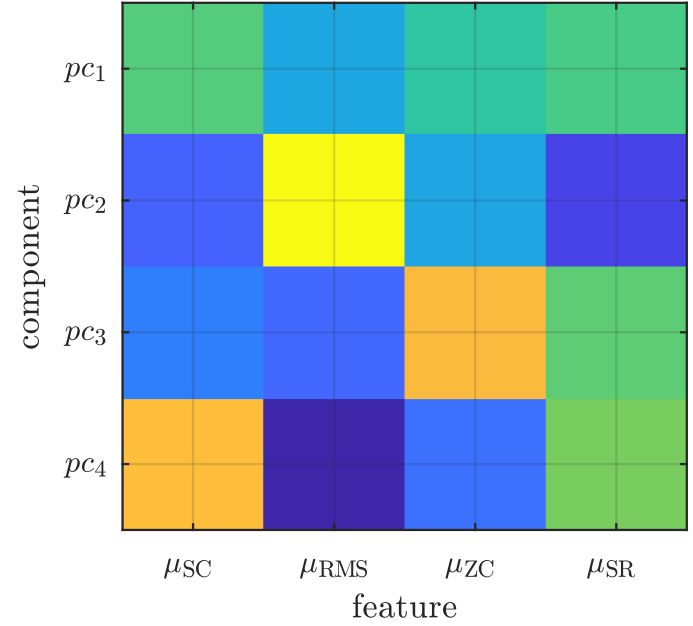
\includegraphics[width=.3
						\columnwidth]{transformation_matrix}%
						\end{figure}
    
\end{frame}


    \section{conclusion}
        \begin{frame}{principal component analysis}{conclusion}
    \begin{itemize}
			\item	\textbf{well-known} tool for dimensionality reduction
			\item widely \textbf{implemented}
			\item \textbf{convenient} characteristics (sorting of components, uncorrelated output)
			\smallskip
			\item<2-> common \textbf{user errors}
				\begin{itemize}
					\item missing or incorrect normalization impacts result
					\item final number of components improperly set
					\item classification tasks: computing the transformation matrix from full data and not training data
				\end{itemize}
			\smallskip
			\item<3-> \textbf{potential problems}
			\begin{itemize}
					\item nonlinear relationships between inputs
					\item interpretability of components
					\item impacted by outliers
			\end{itemize}
		\end{itemize}	
    \inserticon{lightbulb}
\end{frame}

        \section[thanks]{thank you}

  \begin{frame}\frametitle{thank you!}\framesubtitle{~}
        \addreference{\href{https://github.com/alexanderlerch}{github.com/alexanderlerch}}
        
        \begin{block}{links}
            alexander lerch: \href{https://www.linkedin.com/in/lerch}{www.linkedin.com/in/lerch}\\             
            
            \bigskip
            mail: \href{mailto:alexander.lerch@gatech.edu}{alexander.lerch@gatech.edu}

            \bigskip                
            book: \href{https://www.AudioContentAnalysis.org}{www.AudioContentAnalysis.org}
            
            \vspace{-25mm}
            \begin{flushright}
                
\includegraphics[scale=.20]{cover_aca2_thumb}
            \end{flushright}
            \vspace{-15mm}

            %\bigskip
            %zplane.development: 
            %\href{https://www.zplane.de}{www.zplane.de}

            \bigskip
            music informatics group:
            \href{http://musicinformatics.gatech.edu}{musicinformatics.gatech.edu}
                            
            \vspace{5mm}

        \end{block}
        
        \inserticon{mail}
        
    \end{frame}


    %\begin{frame}[allowframebreaks]{references}{references}
        %\printbibliography[title=references]
    %\end{frame}

\end{document}

